    \documentclass[12pt,a4paper]{article}
    \usepackage[T2A]{fontenc}
    \usepackage[utf8]{inputenc}
    \usepackage[russian]{babel}
    \usepackage{amsmath}
    \usepackage{amssymb}
    \usepackage{graphicx}
    \usepackage{floatrow}
    \usepackage{booktabs}
    \usepackage{wrapfig}
    \usepackage{lipsum}
    \usepackage{subcaption}
    \usepackage{fancyhdr}
    \usepackage{mathrsfs}
    \usepackage{tikz}
    
    \newcommand{\figref}[1]{(См. рис. \ref{#1})}
    \newcommand{\secref}[1]{(См. раздел. \ref{#1})}
    
    \newcommand{\e}[1]{\text{$\cdot10^{#1}$}}
    
    \pagestyle{fancy}
    \fancyhead{}
    \fancyhead[L]{Работа 4.4.3}
    \fancyhead[R]{}
    \fancyfoot[C]{\thepage}
    
    \author{\normalsize Выполнил: Голубович Тимур, группа Б01-108 \\
    	\normalsize 05.11.2022}
    \date{}
    
    \usepackage{float}
    \restylefloat{table}
    \title{
    	\large Отчет о выполнении лабораторной работы 4.4.3 \\
    	\Large Изучение призмы с помощью гониометра\\ 
    }
    
    \begin{document}
    	\maketitle
    	
    \section*{Цель работы}
    Знакомство с работой гониометра, исследование дисперсии стеклянной призмы и определение характеристик призмы как спектрального прибора.
    
    
    \section*{Оборудование и приборы} 
    Гониометр;
    ртутная лампа;
    призма;
    стеклянная плоскопараллельная пластинка;
    призменный уголковый отражатель.

	
	\section*{Теоретическое введение} 

	Гониометр служит для точного измерения углов и находит широкое применение в оптических лабораториях. С помощью гониометра можно определять показатели преломления и преломляющие углы призм и кристаллов, исследовать параметры дифракционных решёток, измерять длины волн спектральных линий и т. д. В настоящей работе прибор применяется для исследования дисперсии стеклянных призм — зависимости показателя преломления от длины волны.

 	\begin{figure}[h]
		\begin{center}
			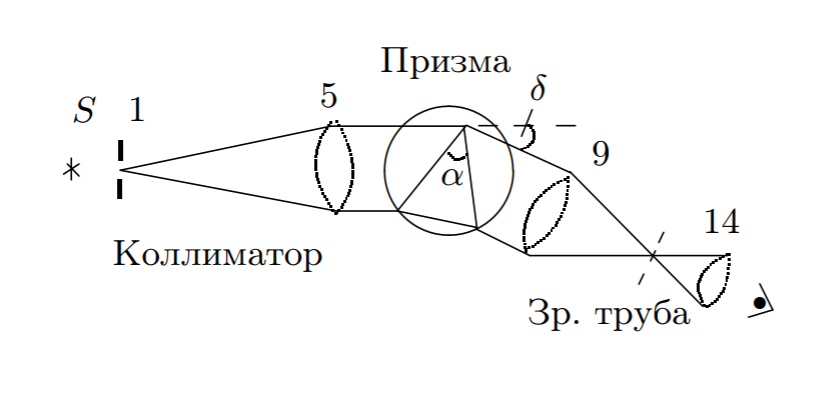
\includegraphics[width = 0.55\textwidth]{res/scheme.png}
			\caption{Оптическая схема эксперимента}
		\end{center}
	\end{figure}
	
	Угол минимального отклонения $\delta$, преломляющий угол $\alpha$ и показатель преломления $n$ связаны между собой соотношением:
	\begin{equation}
		n = \frac{\sin{\frac{\alpha + \delta}{2}}}{\sin{\frac{\alpha}{2}}}
        \label{eq:1}
	\end{equation}

	Измерив с помощью гониометра преломляющий угол призмы и углы наименьшего отклонения для света разных длин волн, можно рассчитать величину $n$ и построить дисперсионную кривую — график зависимости $n(\lambda)$.
	
	По дисперсионной кривой могут быть определены такие важные характеристики оптических стёкол, как средняя дисперсия:
	\begin{equation}
		D = n_F - n_C
        \label{eq:2}
	\end{equation}

	и коэффициент дисперсии $\nu$:
	\begin{equation}
		\nu = \frac{n_D - 1}{n_F - n_C}
        \label{eq:3}
	\end{equation}

	Здесь $n_D$, $n_F$ и $n_C$ — показатели преломления для $\lambda_D$ = $589.3$ нм (среднее значение длин волн жёлтого дублета натрия), $\lambda_F$ = $486.1$ нм (голубая линия водорода), $\lambda_C$ = $656.3$ нм (красная линия водорода).
	
	По наклону дисперсионной кривой можно оценить разрешающую способность призмы:
	\begin{equation}
		R = \frac{\lambda}{\delta \lambda} = b\frac{dn}{d\lambda}
	\end{equation}

 
	\section*{Экспериментальная установка}

    \begin{figure}[h]
		\begin{center}
			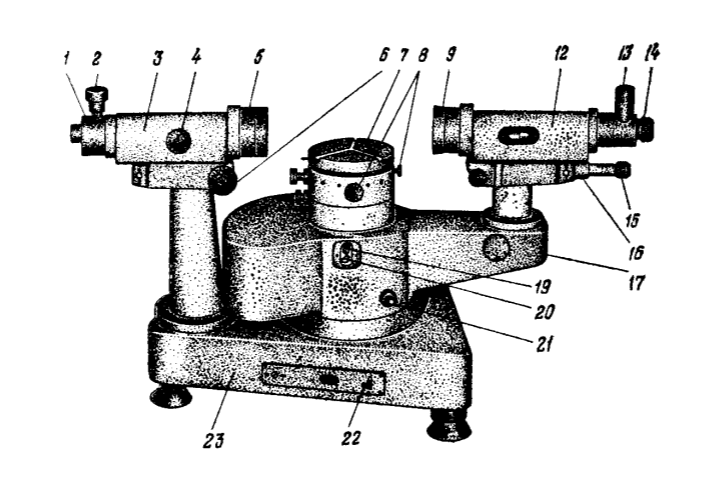
\includegraphics[width = 0.9\textwidth]{res/goniometr.png}
			\caption{Внешний вид гониометра}
            \label{fig:gon}
		\end{center}
	\end{figure}

 	Оптическая схема гониометра представлена на рис. \ref{fig:gon}. Свет от источника $S$ проходит через коллиматор и преобразуется призмой или решёткой в набор параллельных пучков, каждый из которых соответствует определённой длине волны. Параллельные пучки собираются в фокальной плоскости объектива 9 зрительной трубы и рассматриваются глазом через окуляр 14.
	
	Внешний вид гониометра представлен на рис. 1б и 1в. Коллиматор 3, столик 7 и алидада 17 со зрительной трубой 12 крепятся на массивном основании 23. На столике 7 размещаются исследуемые объекты. Коллиматор закреплён неподвижно, а столик и алидада с трубой могут вращаться вокруг вертикальной оси.
	
	Важнейшим узлом гониометра является устройство, служащее для отсчёта угла поворота зрительной трубы вокруг вертикальной оси, проходящей через центр столика. На этой оси крепится прозрачное кольцо (лимб), расположенное в корпусе прибора. На поверхности лимба нанесена шкала с делениями. На поверхности лимба нанесена шкала с делениями. Лимб разделён на $3 \times 360 = 1080$ делений. Цена деления 200, оцифровка делений произведена через $1^\circ$. Шкалу лимба можно наблюдать через окуляр отсчётного устройства 16 при включённой подсветке (тумблер 22). Резкость изображения шкалы регулируется вращением оправы окуляра 15.
	
	Оптическая система отсчётного устройства собрана так, что через окуляр можно наблюдать изображения штрихов двух диаметрально противоположных участков лимба, причём одно изображение прямое, а другое обратное. Кроме того, оптическая система позволяет перемещать эти изображения друг относительно друга, оставляя в покое как лимб, так и алидаду со зрительной трубой.
	
	В работе предлагается отъюстировать гониометр, определить преломляющий угол призмы, измерить углы наименьшего отклонения для нескольких спектральных линий ртути и оценить спектральные характеристики призмы.
	

    \section*{Ход работы}

    \subsection*{Измерение преломляющего угла}

	Для измерения преломляющего угла призмы установим трубу перпендикулярно одной из её отражающих граней и снимем отсчёт по лимбу $\alpha_1 = 72^\circ 23'49''$. Затем, не трогая призму и столик, повернем алидаду с трубой вокруг преломляющего угла призмы и проведем ту же операцию для другой рабочей грани. Получим значение $\alpha_2 = 193^\circ 5'22''$. По углу поворота трубы рассчитаем преломляющий угол призмы:
 
	$$\alpha = \pi - \alpha_1 - \alpha_2 = 59^\circ 18'27''.$$

	\subsection*{Минимальный угол отклонения}

	Для определения минимального угла отклонения $\delta$ поставим призму на столике так, чтобы её основание было параллельно оси коллиматора. Расположим лист бумаги за призмой и найдем на нём спектр, вращая столик рукой. Продолжая поворачивать столик и наблюдая за перемещением спектра, найдем положение столика с призмой, соответствующее минимальному отклонению преломленного луча от направления падающего луча. Измеренные значения углов $\delta$ запишем в таблицу \ref{tab:t1}:
	
    \begin{table}[H]
	   \centering
	   \footnotesize
	   \begin{tabular}{cc}
\toprule
$U_p$, В & $I_p$, мА \\
\midrule
36.25 & 0.20 \\
35.14 & 0.40 \\
33.87 & 0.60 \\
33.03 & 0.80 \\
32.49 & 1.00 \\
32.06 & 1.20 \\
31.76 & 1.40 \\
31.06 & 1.60 \\
30.04 & 1.80 \\
29.63 & 2.00 \\
29.03 & 2.20 \\
28.53 & 2.40 \\
28.04 & 2.60 \\
27.74 & 2.80 \\
27.53 & 3.00 \\
27.39 & 3.20 \\
27.26 & 3.40 \\
27.11 & 3.60 \\
27.08 & 3.80 \\
27.06 & 4.00 \\
27.11 & 4.20 \\
27.12 & 4.40 \\
27.06 & 4.60 \\
27.04 & 4.80 \\
\bottomrule
\end{tabular}

	   \caption{Результаты измерения и обработки минимальных углов отклонения $\delta$}
	   \label{tab:t1}
    \end{table}

	Для оценки разрешающей способности призмы измерим угловую ширину одной из желтых линий дублета, предварительно установив минимально возможную ширину входной щели: $\Delta \delta = 39''$. 
	
	Измерим линейкой длину основания призмы: $b = (7.5 \pm 0.1)$ см.
	
    Рассчитаем показатель преломления $n(\alpha, \delta)$ по формуле \ref{eq:1}. Результаты заносим в таблицу \ref{tab:t1}:

	Теперь построим дисперсионную кривую $n(\lambda)$.
    \begin{figure}[H]
    	\centering
    	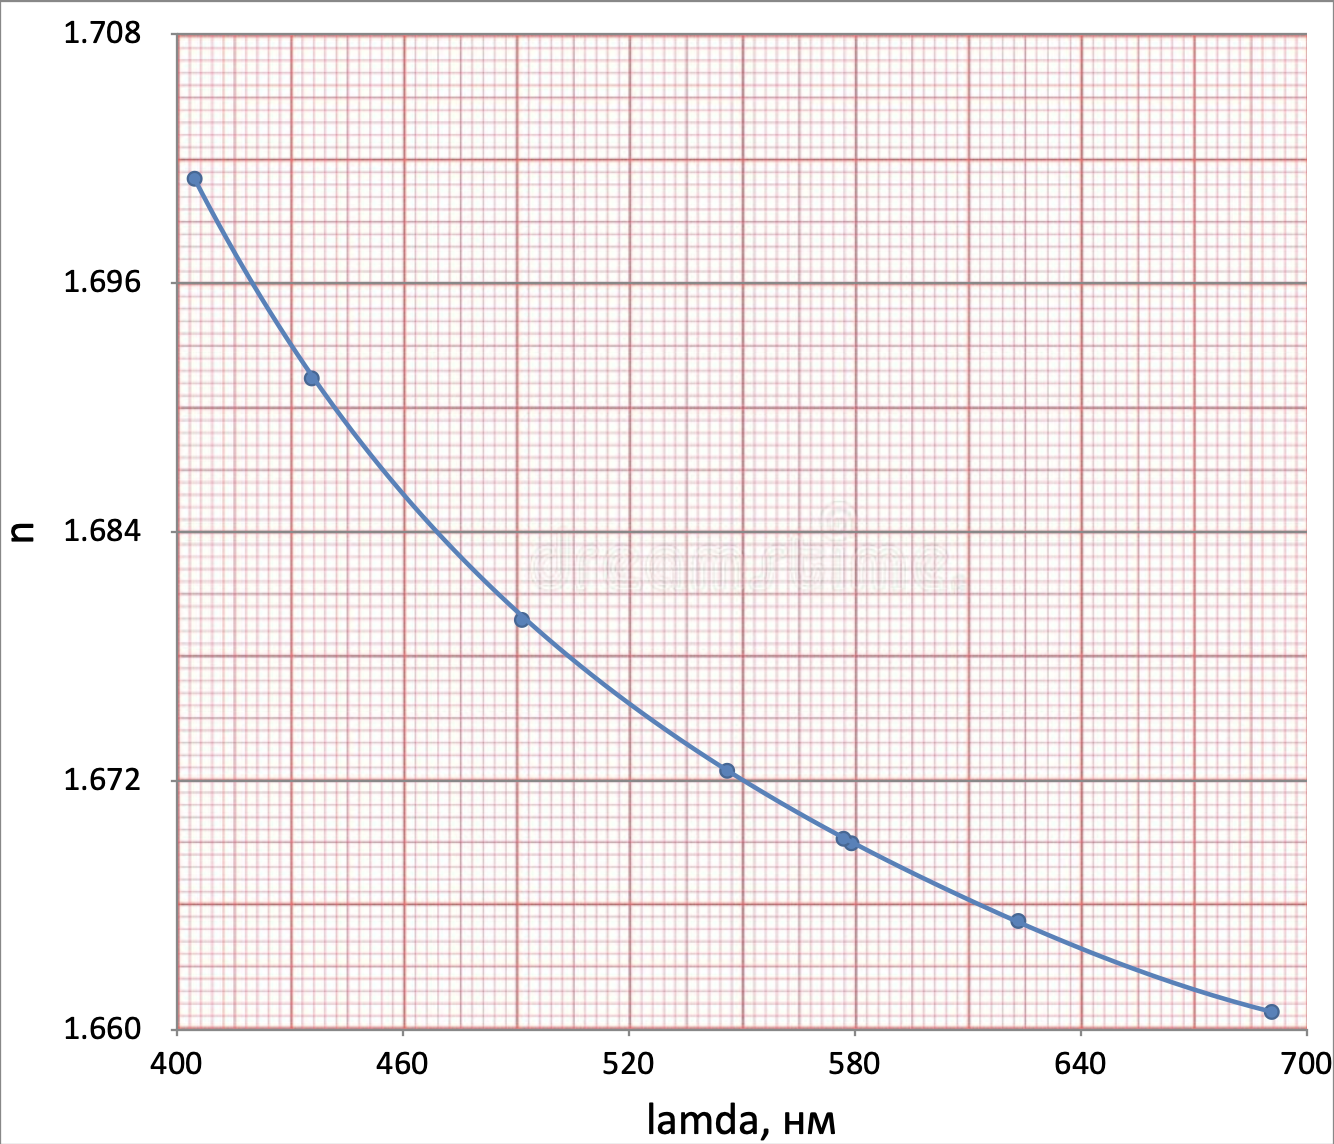
\includegraphics[width=10cm]{src/n_lambda.png}
    	\caption{Дисперсионная кривая}
    	\label{fig:disp}
    \end{figure}
	
	Погрешность $\sigma_n = 0.002$ везде.

    В качестве дополнительного задания проверим формулу Коши аппроксимации зависимости показателя преломления среды от длины волны:

    \begin{equation}
        n = a + b/\lambda^2.
        \label{eq:5}
    \end{equation}

    Построим график $n(\lambda^{-2})$ и рассчитаем параметры $a$ и $b$.

    \begin{figure}[H]
    	\centering
    	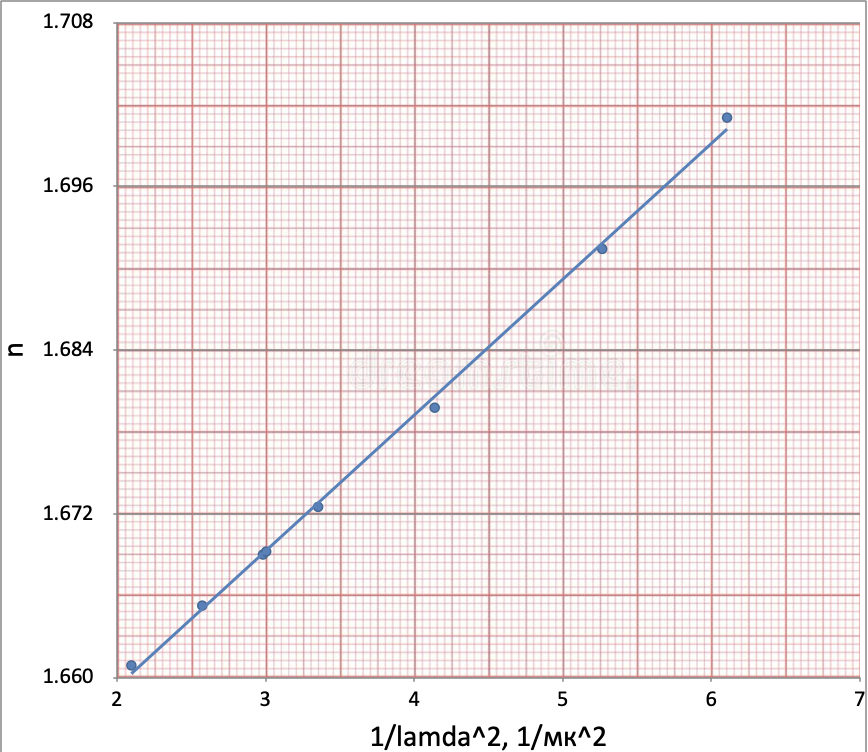
\includegraphics[width=10cm]{src/n_lambda^-2.png}
    	\caption{График $n(\lambda^{-2})$ для проверки формулы Коши}
    	\label{fig:koshi}
    \end{figure}

	Определим по графику $n_D$, $n_F$ и $n_C$. Получаем значения:
    $$ a = 9.95 \pm 0.3 \cdot 10^{-15} \; \text{м}^{-2} \;\;\; \varepsilon_a = 3\% $$
    $$ b = 1.6394 \pm 0.0013 \;\;\; \varepsilon_b = 0.08\% $$
    Погрешности $a$ и $b$ очень маленькие, следовательно формула \ref{eq:5} отлично выполняется в соответсвующем диапазоне длин волн.
	
	\begin{equation*}
		n_D = (1.668 \pm 0.002) \hspace{10mm} n_F = (1.682 \pm 0.002) \hspace{10mm} n_C = (1.663 \pm 0.002) 
	\end{equation*}

	Теперь рассчитаем среднюю дисперсию $D = n_F - n_C$:
	\begin{equation*}
		\boxed{D = (0.019 \pm 0.003)}
	\end{equation*}

	И число Аббе по формуле \ref{eq:3}:
	\begin{equation*}
		\boxed{\nu = (35 \pm 6)}
	\end{equation*}

    \begin{figure}[h]
		\begin{center}
			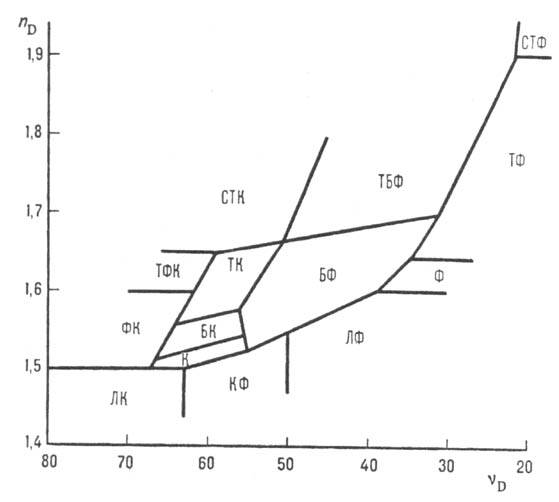
\includegraphics[width=7cm]{res/abbe.jpg}
			\caption{Диагамма Аббе}
            \label{fig:abe}
		\end{center}
	\end{figure}

	Из диаграммы видно, что в данном эксперименте стекло из сорта баритового флинта.
	
	
	По наклону кривой $dn/d\lambda$ рассчитаем максимальную разрешающую способность призмы:
	\begin{equation*}
		R = b\frac{dn}{d\lambda}.
	\end{equation*}	
	
	Из графика получаем, что:
	\begin{equation*}
		\left(\frac{dn}{d\lambda}\right)_{\text{max}} = (31 \pm 5) \cdot 10^{-5} \text{ нм}^{-1} = (31 \pm 5) \cdot 10^2 \text{ см}^{-1}.
	\end{equation*}

	Тогда максимальная разрешающая способность:
	\begin{equation*}
		\boxed{R = (23250 \pm 3800)}
	\end{equation*}

	Рассчитаем экспериментальную величину $R$ по измерениям желтого дублета:
	\begin{equation*}
		\boxed{R = \frac{\lambda}{\delta \lambda} = 560}
	\end{equation*}

	Оценим, при каком размере решетки, имеющей $d^{-1} = 100$ штр/мм, она обладает такой же разрешающей способностью в первом порядке, как призма с основанием $b = 5$ см:
	\begin{equation*}
		a\cdot 100 = b\frac{dn}{d\lambda}
	\end{equation*}
	Откуда получаем $a = (155 \pm 25)$ мм.
	
	Рассчитаем угловую дисперсию $d\varphi/d\lambda$ по измерениям желтого дублета:
	\begin{equation*}
		\frac{d\varphi}{d\lambda} = \frac{\delta_{\text{желт}_1} - \delta_{\text{желт}_2}}{\lambda_{\text{желт}_1} - \lambda_{\text{желт}_2}}
	\end{equation*}

	Получаем следующее значение:
	\begin{equation*}
		\boxed{\frac{d \varphi}{d \lambda} = (182 \pm 3) \cdot 10^{-6} \; \frac{\text{рад}}{\text{нм}} = (182 \pm 3) \text{ мм}^{-1}}
	\end{equation*}

	И теперь сравним её с дисперсией решетки в первом порядке, имеющей $d^{-1} = 100$ штр/мм:
	\begin{equation*}
		\boxed{\frac{d \varphi}{d \lambda} \approx \frac{1}{d} = 100 \text{ мм}^{-1}}
	\end{equation*}
	
	Как видим, дисперсия, измеренная по дублету, и дисперсия решетки имеют одинаковый порядок, однако у дублета она в $\thicksim 2$ раза больше. 
	
	
	\section*{Вывод}
	Самым главным в этой работе стало знакомство с работой гониометра. В дополнение к этому мы провели исследование дисперсии стеклянной призмы и определили характеристики призмы как спектрального прибора:
	\begin{equation*}
		n_D = (1.668 \pm 0.002) \;\;\; n_F = (1.682 \pm 0.002) \;\;\; n_C = (1.663 \pm 0,002) \;\;\; \varepsilon_n = 0.13 \; \%;
	\end{equation*}

\noindent	Средняя дисперсия:
	
\noindent	$D = (0.019 \pm 0.003) \;\;\; \varepsilon_D = 16 \; \%$;

\noindent	Число Аббе:
	
\noindent	$\nu = (35 \pm 6) \;\;\; \varepsilon_{\nu} = 15 \; \%$;

\noindent	Экспериментальная разрешающая способность:
	
\noindent	$R = 560$;
	
\noindent	Угловая дисперсия:
	
\noindent	$\frac{d \varphi}{d \lambda} = (182 \pm 3) \text{ мм}^{-1} \;\;\; \varepsilon_{\frac{d \varphi}{d \lambda}} = 1.6 \; \%$.

\vspace{5mm}

	Как видно, ошибки небольшие и максимальная составляет $\thicksim 17\%$. Все эти ошибки связаны с неточностью измерений и несовершенством техники ее проведения.

\newpage
\begin{thebibliography}{9}
	\bibitem{Siv} Сивухин Д. В. \emph{Общий курс физики. Том 4 Оптика}, 2004
	\bibitem{kirich} Кириченко Н.А. \emph{Оптика.}, 2011
	\bibitem{max} \emph{Лабораторный практикум по общей физике. В 3 томах. Том 3. Оптика: учебное пособие} под ред. А. В. Максимычева, М. Г. Никулина
\end{thebibliography}

\end{document}
